\documentclass{article}
\usepackage{amsmath}
\usepackage{algorithm}
\usepackage{algorithmic}
\usepackage{tikz}
\usepackage{amsfonts}
\usepackage{graphicx}

\title{Reinforcement Learning in Hawk-Dove Game with Mutation}
\author{Geoffrey Wang}
\date{August 2024}

\begin{document}

\maketitle

\section{Introduction}
The Hawk-Dove game is a classic model in evolutionary game theory that describes the interactions between two strategies: Hawk and Dove. The Hawk strategy involves aggressive behavior, whereas the Dove strategy involves peaceful behavior. A mixed strategy can also be considered, where individuals probabilistically choose between Hawk and Dove behaviors. Reinforcement Learning (RL) can be used to model how strategies evolve over time based on their payoffs. This document describes the implementation of an RL-based Hawk-Dove game with the inclusion of mutation, which allows strategies to change randomly over generations.

\section{Implementation of the Hawk-Dove Game with RL}

\subsection{Strategy Definition}
We define three strategies: Hawk, Dove, and Mixed, each represented by an integer constant:
\begin{itemize}
    \item Hawk ($H$) is represented by 0.
    \item Dove ($D$) is represented by 1.
    \item Mixed ($M$) is represented by 2.
\end{itemize}

\subsection{Q-Learning Parameters}
The following parameters are used in the Q-learning algorithm:
\begin{itemize}
    \item Learning rate ($\alpha = 0.1$)
    \item Discount factor ($\gamma = 0.95$)
    \item Exploration rate ($\epsilon = 0.1$)
    \item Mutation rate ($\mu = 0.01$)
\end{itemize}

\subsection{Individual Class}
Each individual in the population is represented by an object of the \texttt{Individual} class. This class maintains a Q-table for each strategy and provides methods to choose actions, update Q-values, and mutate strategies.

\begin{algorithm}[H]
\caption{Individual Class Implementation}
\begin{algorithmic}[1]
\STATE Initialize strategy and Q-table
\FUNCTION{choose\_action}{}
    \IF{strategy is MIXED}
        \STATE Choose between HAWK and DOVE based on Q-values
    \ELSE
        \STATE Choose action based on $\epsilon$-greedy policy
    \ENDIF
\ENDFUNCTION
\FUNCTION{update\_q\_value}{action, reward, next\_max\_q}
    \STATE Update Q-value using the Q-learning formula
\ENDFUNCTION
\FUNCTION{mutate}{}
    \STATE Randomly mutate strategy with probability $\mu$
\ENDFUNCTION
\FUNCTION{play}{opponent, V, C}
    \STATE Determine payoffs based on strategies and return them
\ENDFUNCTION
\end{algorithmic}
\end{algorithm}

\subsection{Population Class}
The population is represented by an object of the \texttt{Population} class, which consists of multiple \texttt{Individual} objects. The population evolves over generations based on the Q-learning algorithm and mutation.

\begin{algorithm}[H]
\caption{Population Evolution}
\begin{algorithmic}[1]
\STATE Initialize population with a mix of HAWK, DOVE, and MIXED strategies
\FOR{each generation}
    \STATE Calculate fractions of HAWK, DOVE, and MIXED strategies
    \FOR{each individual}
        \STATE Choose an opponent randomly
        \STATE Play the game and update Q-values
        \STATE Apply mutation to the individual's strategy
    \ENDFOR
    \STATE Normalize the fractions to ensure they sum to 1
\ENDFOR
\end{algorithmic}
\end{algorithm}

\section{Markov Decision Process with Mutation}
The Markov Decision Process (MDP) for this problem involves states corresponding to the strategies (Hawk, Dove, Mixed). The actions are the potential strategies that an individual can choose. The rewards are determined based on the interactions between individuals, and the transitions are governed by the Q-learning algorithm and the mutation mechanism.

\subsection{State Transition Diagram}
The state transition diagram for the Hawk-Dove game with mutation is depicted in Figure \ref{fig:transitions}. The transition probabilities are influenced by the Q-values and the mutation rate. Mutation introduces randomness into the process, allowing strategies to transition even if they are not optimal according to the Q-values.

\begin{figure}[h!]
    \centering
    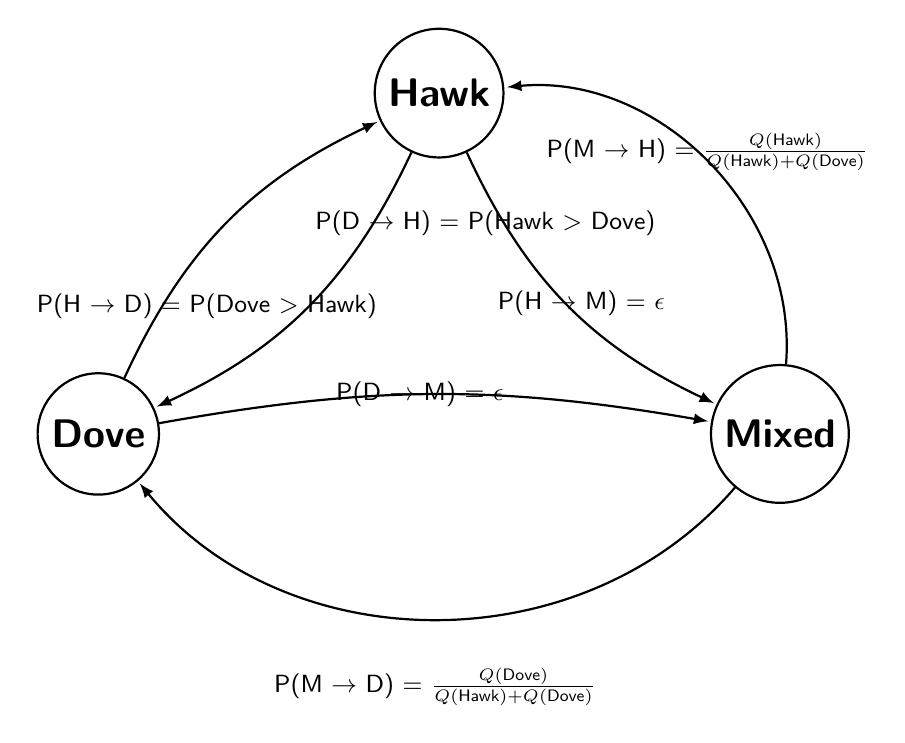
\begin{tikzpicture}[->,>=latex,shorten >=1pt,auto,node distance=4cm, thick,
      main node/.style={circle,draw,font=\sffamily\Large\bfseries}]

      \node[main node] (H) {Hawk};
      \node[main node] (D) [below left of=H, xshift=-1.5cm, yshift=-1.5cm] {Dove};
      \node[main node] (M) [below right of=H, xshift=1.5cm, yshift=-1.5cm] {Mixed};

      \path[every node/.style={font=\sffamily\small}]
        (H) edge [bend left=20] node [left, xshift=1cm] {P(H $\rightarrow$ D) = P(Dove $>$ Hawk)} (D)
            edge [bend right=20] node [right, xshift=-1cm] {P(H $\rightarrow$ M) = $\epsilon$} (M)
        (D) edge [bend left=20] node [right, xshift=1cm] {P(D $\rightarrow$ H) = P(Hawk $>$ Dove)} (H)
            edge [bend left=10] node [left, xshift=1cm] {P(D $\rightarrow$ M) = $\epsilon$} (M)
        (M) edge [bend right=50] node [below, yshift=0.5cm] {P(M $\rightarrow$ H) = $\frac{Q(\text{Hawk})}{Q(\text{Hawk}) + Q(\text{Dove})}$} (H)
            edge [bend left=50] node [below, yshift=-0.5cm] {P(M $\rightarrow$ D) = $\frac{Q(\text{Dove})}{Q(\text{Hawk}) + Q(\text{Dove})}$} (D);
    \end{tikzpicture}
    \caption{Strategy State Transition Diagram with Conditional Probabilities}
    \label{fig:transitions}
\end{figure}

\end{document}
